\subsection{流程控制}

\begin{frame}{流程控制}
    \begin{columns}
        \column{0.6\textwidth}
            \begin{myoutline}
                \1 顺序结构
                \1 分支结构——判断
                    \2 if, if else, if elif else
                \1 循环结构——循环
                    \2 while loop
                    \2 for loop
                \1 练习:九九乘法表
                    \2 if + for loop
            \end{myoutline}

            \begin{figure}
                \centering
                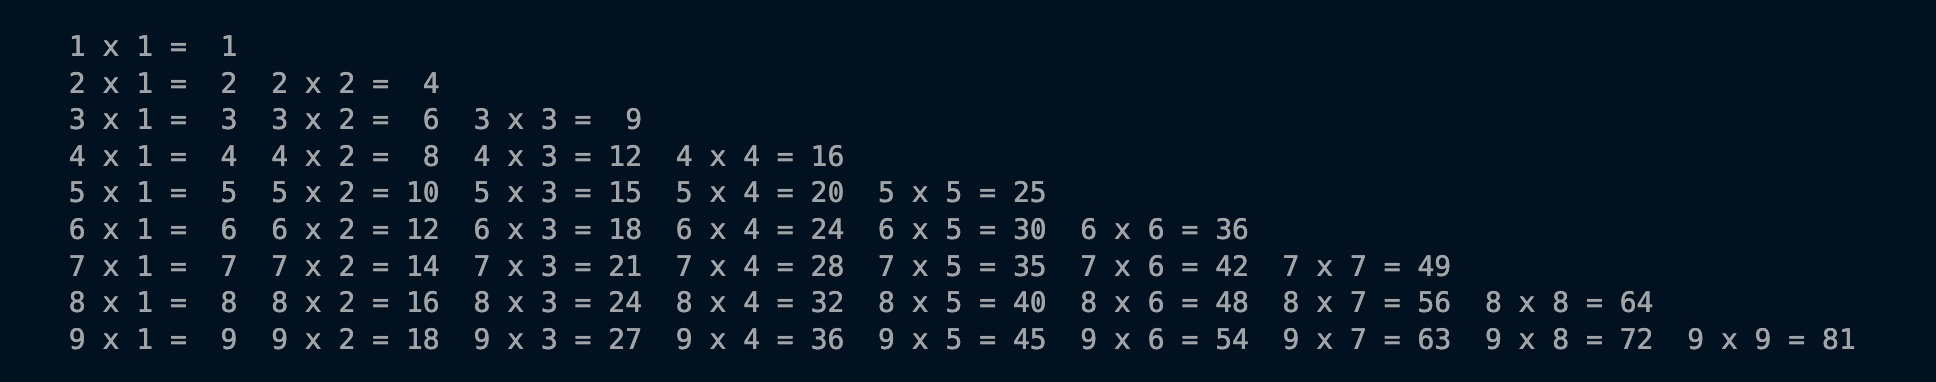
\includegraphics[width=1\linewidth]{Images/99multi.jpg}
            \end{figure}
        \column{0.4\textwidth}
            \begin{figure}
                \centering
                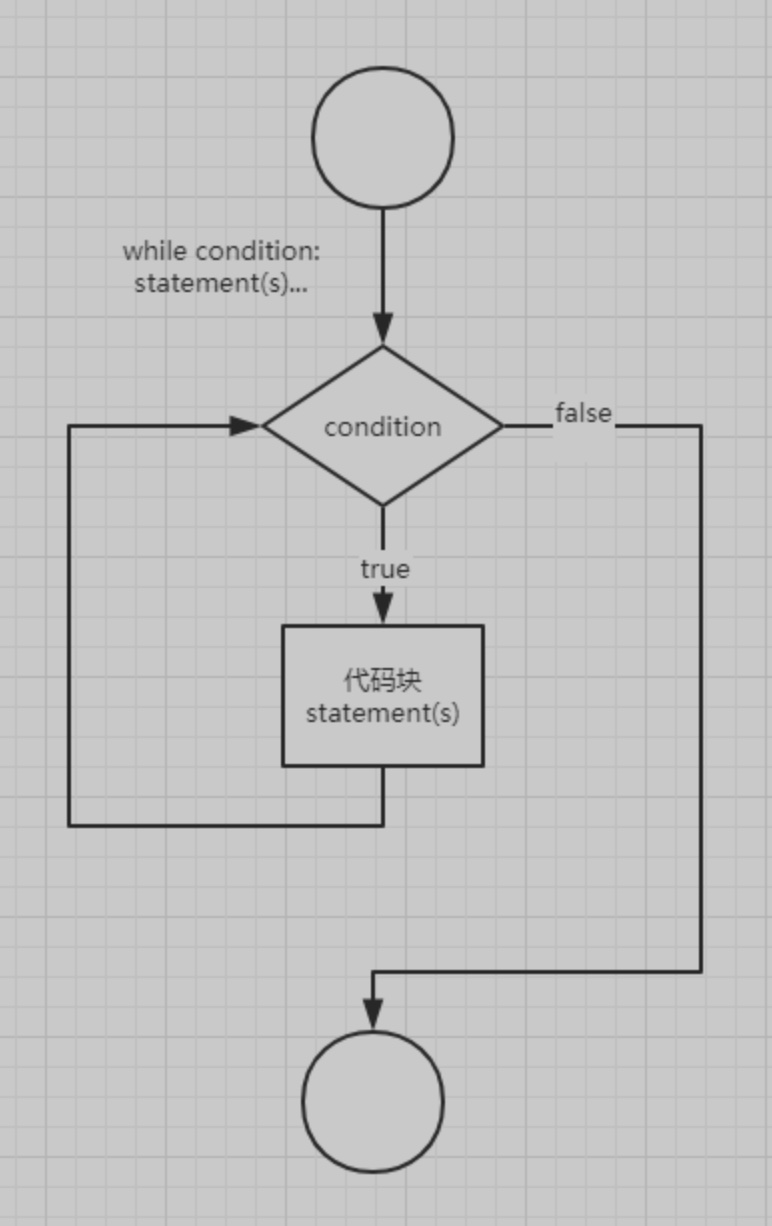
\includegraphics[width=0.7\linewidth]{Images/Loop.jpg}
            \end{figure}
    \end{columns}
\end{frame}